\chapter[Results]{Results}
- For each run there is a subset of models
- For each model there is a subset of scalar values
- For each scalar value there is a subset of plots
- For each subset of plots there are observations of those plots

- For each question there is a subset of models being compared
- For each model being compared there is a subset of scalar values being
differenced
- For each scalar value being differenced there is a plot of the differences
- For each plot of the differences there are observations of those plots

\section[The Reconnecting Magnetosphere]{The Kennel view of the reconnecting
magnetosphere} The following section describes a long supported view of the magnetosphere. The
book ``Convection and Substorms'' by Kennel \cite{Kennel} has a chapter devoted
to a view of the reconnecting magnetosphere. Important to this style of
validation is to have a view of the magnetosphere before viewing the results of
a models output of how it calculates the magnetosphere. A similar structure
should be seen by the models as is portrayed by Kennel. This section will also
contain images from published papers that give a general structure of the B
field, number density and velocities as they change in specific parts of the
magnetosphere.
\begin{figure}
	\centering
	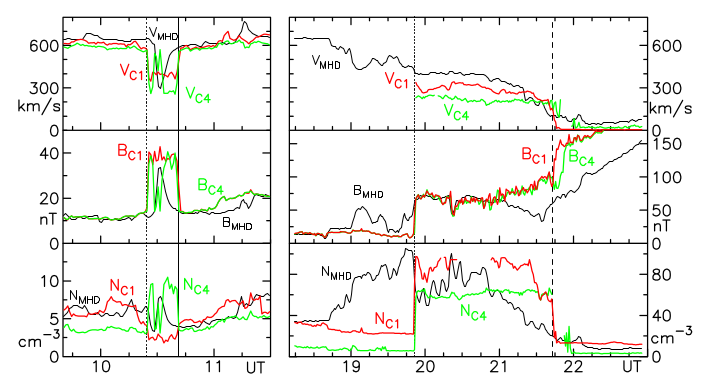
\includegraphics[scale=0.5]{images/MPandShock_VBN.png}
	\caption{Satellite measurements of velocity, magnetic field strength and
	number density taken from Cluster 1 and Cluster 4 instruments as they
	cross through the Earths bow shock and magnetopause.}
    \label{fig:MPandShock_VBN}
	\figSpace
\end{figure}

\begin{figure}
	\centering
	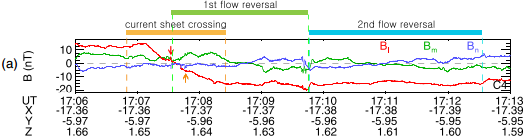
\includegraphics[scale=0.75]{images/Cur_sheet_B.png}
	\caption{Cluster 4 measurements of magnetic field strength as it crosses the
	current sheet in the magnetotail with time on the x axis.}
    \label{fig:Cur_sheet_B}
	\figSpace
\end{figure}

\begin{figure}
	\centering
	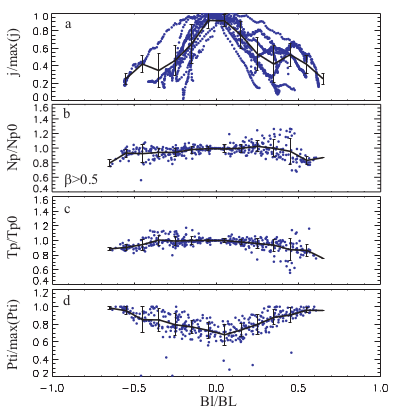
\includegraphics[scale=0.75]{images/Cur_sheet_N.png}
	\caption{Profiles of the current density (a), proton number density,
normalized by the value N0 =Np (Bl =0) (b), and proton tempera-
ture (c) normalized by T0 =Tp (Bl =0), and the sum of magnetic and
ion pressures (P ti ) (d), normalized by their maximum value, versus
normalized main magnetic field Bl /BL for class I current sheets.
}
    \label{fig:Cur_sheet_N}
	\figSpace
\end{figure}
At the bow shock(heading towards the Earth) based on a paper from Tatrallyay
\cite{Tatrallyay2012} and seen in Figure \ref{fig:MPandShock_VBN}, There is a
velocity decrease at the bow shock and a decrease at the magnetopause, a total B increase at both the bow shock and magnetopause, density
increase at the bow shock and density decrease at the magnetopause.
At the magnetotail crossing, based on papers by Runov \cite{Runov2006}, and
Hwang \cite{Hwang2013} there is a velocity increase as the distance to the
current sheet decreases. The magnetic field decreases and reverses direction as the current
sheet is crossed as seen in Figure \ref{fig:Cur_sheet_B}. The number density
increases as the distance to the current sheet decreases as seen in Figure
\ref{fig:Cur_sheet_N}.
The following relates the satellite observations with the general understanding
of the reconnecting magnetosphere as described by Kennel (1995).
\begin{itemize}
	\item Total B
	\begin{itemize}
		\item Due to the direction of the Earth's magnetic dipole at the magnetopause
		being similar to the IMF there is a buildup of magnetic field. This buildup is
		between the magnetopause and the bow shock.
		\item Due to the enhancement of Bz sunward, the magnetopause will
		move sunward.
		\item With a negative Bz, the IMF and Earths dipole would oppose each
		other and degrade the magnetic field at the magnetopause causing the dipole
		field lines to reconnect with the IMF and travel tailward giving the
		magnetotail the appearance of enlarging. Since the magnetic field is more
		mobile around the magnetosphere with the reconnection, the buildup of magnetic
		field at the tip of the magnetopause will decay.
		\item Due to the degrade of Bz at the magnetopause, the magnetopause will
		move Earthward.
		\item There will be a high total B around Earth as the Earths dipole is
		much stronger than the IMF at the Earth.
		\item Because of the stretching of the magnetic field in the magnetotail the
		strength of the magnetic field in the current sheet region goes to zero as
		the stretching causes oppositely directed magnetic fields to draw closer and
		cancel one another out.
	\end{itemize}
	
	\item rho
	\begin{itemize}
		\item The plasma that travels along with the IMF has many variables associated
		with is and one of the measured variables is density. As stated in the Total B
		case, for positive Bz cases where there is a build up of magnetic field at
		the magnetopause, there will also be a build up of density. This will also be
		between the bow shock and the magnetopause.
		\item Based on Petschek's steady reconnection model, due to the
		stretching of magnetic field in the magnetotail there are regions where
		oppositely directed magnetic field lines can get close enough to one
		another and reconnect. This plane is called the plasma sheet and it separates
		the two opposing magnetic field directions. When reconnection occurs there, a
		flow of plasma needs to replace the plasma loss and creates a build up of
		plasma leading to a gradual increase of density in the current sheet.
		\item The are three motions of the plasma particles as they travel in the
		magnetosphere. There is a particle rotation around magnetic field lines, a
		bounce motion from pole to pole and a magnetic field rotational aspect around
		the Earth. The pole to pole bounce motion will cause a build up of plasma
		density closer to the Earth dependant on the energies of the
		particles in the plasma. 
	\end{itemize}
	
	\item Ux
	\begin{itemize}
		\item The velocity of the plasma from the solar wind is supersonic. Inside the
		magnetosphere there is very little in the way of solar wind velocity. As the
		solar wind is slowed down by the magnetosphere there is a point in which the
		solar wind velocity switches from supersonic to subsonic. This region is known
		as the bow shock.
		\item Because the magnetic field of the Earth is much stronger than the IMF,
		the velocities in the magnetosphere are almost zero. Due to this, there would
		be a second drop off of solar wind velocity at the magnetopause.
		\item With the reconnection in the magnetotail occurring in the plasma sheet,
		there is a push of plasma both towards and away from the Earth on each side of
		where the reconnection occurred. This movement is the reason that increases in
		velocities are seen as your distance from the plasma sheet neutral line
		decreases.
	\end{itemize}
\end{itemize}

Keeping to generic observational differences and getting more specific will be
the method used in the following sections. Starting with generic observation,
when viewing the output from models a first comparison should be made between
the view portrayed by Kennel and the view portrayed by the image created from
the models output data. To get more specific, the view portrayed by the
difference output plots will be used.
\section{Pre-Conditioning}
For the first two runs, there are two different time periods in which the
generic view of the magnetosphere will change. First the period of time before
the Bz flip occurs where the magnetic field of the IMF is the same direction as
the Earths and secondly the period of time after the Bz flip where the direction
of the IMF is opposite to that of the earths and the shape of the magnetosphere
will change.
\begin{figure}
	\centering
	\includegraphics[scale=0.45]{images/R1M1B6crop_alpha.png}
	\caption{OpenGGCM Total B scalar field output viewed on the X-Z plane with the
	X and Z in Earth radii. }
    \label{fig:R1M1B6crop}
	\figSpace
\end{figure}
Looking at the OpenGGCM output before the Bz flip, The first scalar field
plotted is the Total B field. All features of the B field match the view portrayed in the
literature. Looking at figure \ref{fig:R1M1B6crop}, the magnetopause has an
increase of B ahead of it as the IMF B is piling up then a secondary increase inside of
the magnetopause. Looking in the current sheet region the B field also goes to
zero as the middle of the current sheet is reached.
\begin{figure}
	\centering
	\includegraphics[scale=0.45]{images/R1M1rho6crop.png}
	\caption{OpenGGCM scalar rho field output viewed on the X-Z plane with the
	X and Z in Earth radii. }
    \label{fig:R1M1rho6crop}
	\figSpace
\end{figure}
The next plot is of the scalar field rho which is a number density which can
be seen in figure \ref{fig:R1M1rho6crop}. The density in the current
sheet cannot be seen because it's too low for the plot range to pick up on. It
can been made easier to see with more colors, but important features would blend
together and become more difficult to identify. Also, there should be a higher density 
around Earth but this is not seen. The high density seen sunward of the
magnetopause agrees with the image portrayed by Kennel.
\begin{figure}
	\centering
	\includegraphics[scale=0.45]{images/R1M1Ux6crop.png}
	\caption{OpenGGCM scalar velocity field output viewed on the X-Z plane with the
	X and Z in Earth radii. }
    \label{fig:R1M1Ux6crop}
	\figSpace
\end{figure}
In the velocity images, the magnetopause and bow shock region agree with
satellite measurements in that there are two significant flow decreases as
you traverse towards the Earth from the Sun. There are two interesting features
First there appears to be a cascading reconnection in flow as it travels
tail ward starting around the tail region x-line. Second there is an Earthward
flow in the tail region between 50-80Re that appears to be there for the entire
run, the change is in it's intensity.
\begin{figure}
	\centering
	\includegraphics[scale=0.45]{images/R1M1B13crop.png}
	\caption{OpenGGCM scalar total B field output viewed on the X-Z plane with the
	X and Z in Earth radii. }
    \label{fig:R1M1B13crop}
	\figSpace
\end{figure}
After the Bz flip as seen in figure \ref{fig:R1M1B13crop}, the region ahead of
the magnetopause where there was a buildup of B is much smaller. As the magnetic
field at the magnetopause gets reconnected to the IMF and travels tailward, the
buildup of B ahead of the magnetopause will travel with the reconnected field in
the IMF tailward helping to give it a compressed look. The movement of B from
the magnetopause into the outer tail region gives the tail a higher B further
from the current sheet region.

\begin{figure}
	\centering
	\includegraphics[scale=0.45]{images/R1M2rho1crop.png}
	\caption{BATS-R-US scalar density output viewed on the X-Z plane with the
	X and Z in Earth radii. }
    \label{fig:R1M2rho1crop}
	\figSpace
\end{figure}
Next, looking at the BATS-R-US model, the features that are portrayed in the
literature match to what was seen in the scalar B field and the scalar
velocity. The scalar density has new features that were not seen in the OpenGGCM
model that match better to what the literature portrays. First there is a hint
that there are higher densities in the current sheet region as seen in figure
\ref{fig:R1M2rho1crop}, as well as the region around the Earth has a higher
density.
There is a noticeable difference in the velocities in the current sheet region
between the BATS-R-US and the OpenGGCM in that the OpenGGCM appears to have a
bursty convection throughout the entire run in the current sheet while the
BATS-R-US has a tailward velocity that stabilizes as time progresses forward, as
seen in figure \ref{fig:R1M2Ux31crop}.
\begin{figure}
	\centering
	\includegraphics[scale=0.45]{images/R1M2Ux31crop.png}
	\caption{BATS-R-US scalar velocity output viewed on the X-Z plane with the
	X and Z in Earth radii. }
    \label{fig:R1M2Ux31crop}
	\figSpace
\end{figure}

Nothing in the SWMF run had any substantial differences from what is portrayed
by Kennel. All three scalars agree with what Kennel portrays.

The second run, which moves the Bz flip to later in the time series does not
show anything substantial from what is portrayed by Kennel or what is shown from
the first set of runs where the Bz flip was earlier in the time series.

\section{Extreme events}
\subsection{High Magnetospheric Compression}
In the next two sections the goal is to test the models ability to handle two
extreme conditions. The idea behind a \texit{parameter variability} validation is that
the event type does not necessarily have to have the fluctuations in input that
is seen from satellite measurements, but something that can potentially happen.
For the first model run with extreme conditions, a high compression of the
magnetosphere is looked at.
\begin{figure}
	\centering
	\includegraphics[scale=0.45]{images/R3M1B3crop.png}
	\caption{OpenGGCM scalar total magnetic field output viewed on the X-Z plane
	with the X and Z in Earth radii. }
    \label{fig:R3M1B3crop}
	\figSpace
\end{figure}
In the OpenGGCM model, it appears that all scalar outputs looks normal at the
beginning of the run. As time progresses the model appears to lose stability in
the current sheet region. First, looking at the B field at the beginning of the
run as seen in figure \ref{fig:R3M1B3crop} everything is as it showed in the
previous two models runs where there was some bursty convection in the current sheet region.
The difference is towards the end of the run where there is a different B
structure close to the Earth in the current sheet region as seen in figure
\ref{fig:R3M1B72crop}.
\begin{figure}
	\centering
	\includegraphics[scale=0.45]{images/R3M1B72crop.png}
	\caption{OpenGGCM scalar total magnetic field output viewed on the X-Z plane
	with the X and Z in Earth radii. }
    \label{fig:R3M1B72crop}
	\figSpace
\end{figure}
\begin{figure}
	\centering
	\includegraphics[scale=0.45]{images/R3M1Ux3crop.png}
	\caption{OpenGGCM scalar velocity output viewed on the X-Z plane
	with the X and Z in Earth radii. }
    \label{fig:R3M1Ux3crop}
	\figSpace
\end{figure}
There is nothing that disagrees with Kennel in the scalar density plots, and the
scalar velocity plots show a similar region of interest as the scalar total B
field. The scalar velocity show similarities with how the first model run with
OpenGGCM appeared where there was a bursty tailward flow in the current sheet
region as seen in figure \ref{fig:R3M1Ux3crop}, and what is similar to the
scalar total B field is the region where things change significantly. Looking at
figure \ref{fig:R3M1Ux72crop} in the current sheet region closest to Earth there
is a build up of Earthward velocities that matches the location of the B
buildup seen.
\begin{figure}
	\centering
	\includegraphics[scale=0.45]{images/R3M1Ux72crop.png}
	\caption{OpenGGCM scalar velocity output viewed on the X-Z plane
	with the X and Z in Earth radii. }
    \label{fig:R3M1Ux72crop}
	\figSpace
\end{figure}

\begin{figure}
	\centering
	\includegraphics[scale=0.45]{images/R3M2B6crop.png}
	\caption{BATS-R-US magnetic field output viewed on the X-Z plane
	with the X and Z in Earth radii. }
    \label{fig:R3M2B6crop}
	\figSpace
\end{figure}
The BATS-R-US model has some intriguing features in this case. The first thing
that was identified is a large area of zero B in the distant current sheet
region as seen in figure \ref{fig:R3M2B6crop}. This large area of zero B has the
appearance of moving tailward until approximately timestep number 19 to which
any movement in the model is gone. All scalar fields have the same stop in
movement around the 19th timestep.

\begin{figure}
	\centering
	\includegraphics[scale=0.45]{images/R3M3B6crop.png}
	\caption{SWMF magnetic field output viewed on the X-Z plane
	with the X and Z in Earth radii. }
    \label{fig:R3M3B6crop}
	\figSpace
\end{figure}
The SWMF, in which for the magnetosphere the BATS-R-US is used with the RCM
added, does not appear to stop like the BATS-R-US. There is no large region of
zero B in the distant tail region that moves tailward. A smaller region of zero
B is present as seen in figure \ref{fig:R3M3B6crop}. The B field then appears to
widen and eventually will appear to fluctuate as waves all the way through the
end of the run. All scalar fields have the appearance of fluctuating as waves
all the way through the end of the run.

\subsection{Low Magnetospheric Compression}

Run 4 Model 1
The approximate zero B in the distant tail current sheet region expands through
the run. Everything else seems okay.
Nothing substantial for density
Nothing substantially different from previous runs for velocity.

Run 4 Model 2
Nothing substantial, almost no movement in the model for B.
Same as B, no movement, nothing substantial for density.
Same as B and Rho, no movement nothing substantial for velocity.

Run 4 Model 3
Same as previous Model. maybe a little more movement, but nothing substantial.
Same as B, very little movement, nothing substantial for density
Same as B and density, very little movement and nothing substantial for velocity.




\section{Difference Visualization}
\subsection{Preconditioning}
\subsection{Bz Flip}
\subsection{High Magnetospheric Compression}
\subsection{Low Magnetospheric Compression}
